% Generator: hand-authored TikZ schematic traced from the fixed source-visible prism edges and auxiliary lines; projection is illustrative.
% Source ID: src-96ac0e772a0483bbf7cf803b94b1a1d8d8e1d2ae16b936b196e6abc05d1251ee
% PDF SHA-256: 7e840dc5c259cf05138337178794a58b6593dc7f2bf0d693826489856da416e9
% PDF page 3; question 18.
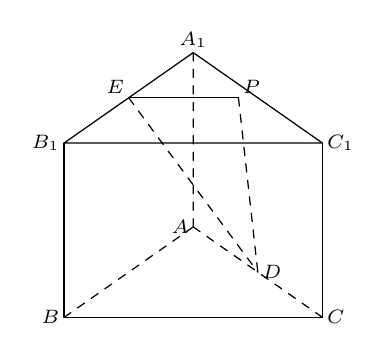
\begin{tikzpicture}[
  x=0.82cm,y=0.82cm,line width=0.45pt,line cap=round,line join=round,
  every node/.style={font=\scriptsize,inner sep=1.5pt}
]
  \coordinate (A)  at (0,-0.2);
  \coordinate (B)  at (-2,-1.6);
  \coordinate (C)  at (2,-1.6);
  \coordinate (A1) at (0,2.5);
  \coordinate (B1) at (-2,1.1);
  \coordinate (C1) at (2,1.1);
  \coordinate (E)  at (-1,1.8);
  \coordinate (D)  at (1,-0.9);
  \coordinate (P)  at (0.7,1.8);

  % Hidden prism edges from the source.
  \draw[dashed] (A)--(B) (A)--(C) (A)--(A1);

  % Auxiliary lines: EP is solid; ED and PD are dashed in the source.
  \draw[dashed] (E)--(D) (P)--(D);
  \draw (E)--(P);

  % Visible prism edges.
  \draw (B)--(C) (B)--(B1) (C)--(C1);
  \draw (A1)--(B1)--(C1)--cycle;

  \node[above] at (A1) {$A_1$};
  \node[left] at (B1) {$B_1$};
  \node[right] at (C1) {$C_1$};
  \node[left] at (B) {$B$};
  \node[right] at (C) {$C$};
  \node[left] at (A) {$A$};
  \node[above left] at (E) {$E$};
  \node[above right] at (P) {$P$};
  \node[right] at (D) {$D$};
\end{tikzpicture}
